% chap11 - Optimization and interpolations
% Last edited:

\chapter{Optimization and interpolation}

\section{ODE Events}
\label{events}

Normally when you call {\tt ode45} you have to specify
a start time and an end time. But in many cases, you don't know ahead
of time when the simulation should end.
Fortunately Octave provides a mechanism for dealing
with this problem. The bad news is that it is a little awkward.
Here's how it works:

\begin{enumerate}

\item Before calling {\tt ode45} you use {\tt odeset} to create an
object called {\tt options} that contains values that control
how {\tt ode45} works:

\begin{verbatim}
options = odeset('Events', @events);
\end{verbatim}
%
In this case, the name of the option is {\tt Events} and the
value is a function handle. When {\tt ode45} runs, it will invoke
{\tt events} after each timestep.
You can call this function anything you want, but the name
{\tt events} is conventional.

\item The function you provide has to take
the same input variables as your rate function. For example,
here is an event function that would work with {\tt projectile}
from Section~\ref{projectile}

\begin{verbatim}
function [value,isterminal,direction] = events(t,X)
  value = X(2);    % Extract the current height.
  isterminal = 1;   % Stop the integration if height crosses zero.
  direction = -1;   % But only if the height is decreasing.
end
\end{verbatim}

{\tt events} returns three output variables:

{\tt value} determines
when an event occurs. In this case {\tt value} gets the second
element of {\tt X}, which is understood to be the height of the
projectile. An ``event'' is a point in time when this value passes
through 0.

{\tt direction} determines whether an event occurs when
{\tt value} is increasing ({\tt direction=1}), decreasing ({\tt
direction=-1}, or both {\tt direction=0}.

{\tt isterminal} determines what happens when an event
occurs. If {\tt isterminal=1}, the event is ``terminal'' and the
simulation stops. If {\tt isterminal=0}, the simulation continues,
but {\tt ode45} does some additional work to make sure that the
solution in the vicinity of the event is accurate, and that one of the
estimated values in the result is at the time of the event.

\item When you call {\tt ode45}, you pass {\tt options} as a fourth
argument:

\begin{verbatim}
ode45(@projectile, [0,10], [0, 3, 40, 30], options);
\end{verbatim}
%
\end{enumerate}

\begin{ex}
How would you modify {\tt events} to stop when the height of
the projectile falls through 3m?
\end{ex}


\section{Optimization}

In Exercise~\ref{baseball}, you were asked to find the optimal
launch angle for a batted ball. ``Optimal'' is a fancy way of
saying ``best;'' what that means depends on the problem. For
the Green Monster Problem---finding the optimal angle for
hitting a home run in Fenway Park, the meaning of ``optimal''
is not obvious.

It is tempting to choose the angle that yields the longest
range (distance from home plate when it lands). But in this
case we are trying to clear a 12m wall, so maybe we want
the angle that yields the longest range when the ball falls
through 12m.

Although either definition would be good enough for most purposes,
neither is quite right. In this case the ``optimal'' angle is
the one that yields the greatest height at the point where
the ball reaches the wall, which is 97m from home plate.

So the first step in any optimization problem is to define
what ``optimal'' means. The second step is to define a range of
values where you want to search. In this case the range of
feasible values is between 0 degrees (parallel to the ground)
and 90 degrees (straight up). We expect the
optimal angle to be near 45 degrees, but we might not be sure
how far from 45 degrees to look. To play it safe, we could
start with the widest feasible range.

The simplest way to search for an optimal value is to run the
simulation with a wide range of values and choose the one
that yields the best result. This
method is not very efficient, especially in a case like this where
computing the distance in flight is expensive.

A better algorithm is a Golden Section Search. 

\section{Golden section search}

To present the Golden Section Search, I will start with a simplified
version I'll call a Silver Section Search. The basic idea is similar to
the methods for zero-finding we saw in Section~\ref{zero}. In the
case of zero-finding, we had a picture like this:

\beforefig \centerline{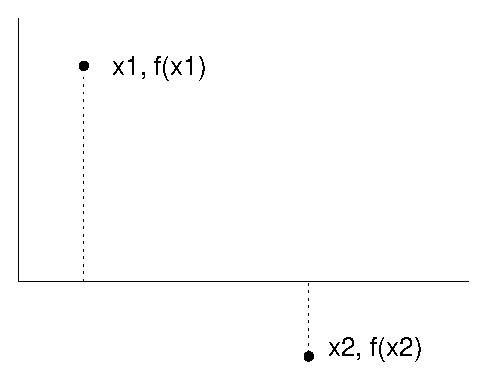
\includegraphics[height=1.5in]{figs/secant.eps}}

We are given a function, $f$, that we can evaluate, and
we want to find a root of $f$; that is, a value of $x$ that makes
$f(x)=0$. If we can find a value, $x_1$, that makes $f(x_1)$ positive
and another value, $x_2$, that makes $f(x_2)$ negative, then there has
to be a root in between (as long as $f$ is continuous). In this
case we say that $x_1$ and $x_2$ ``bracket'' the root.

The algorithm proceeds by choosing a third value, $x_3$, between
$x_1$ and $x_2$ and then evaluating $y = f(x_3)$. If $y$ is
positive, we can form a new pair, $(x_3, x_2)$, that brackets the
root. If $y$ is negative then the pair $(x_1, x_3)$ brackets the root.
Either way the size of the bracket gets smaller, so our
estimate of the location of the root gets better.

So that was root-finding. The Golden Section Search is similar, but
we have to start with three values, and the picture looks like
this:

\beforefig \centerline{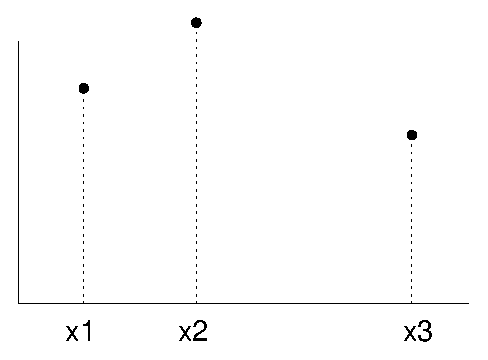
\includegraphics[height=1.5in]{figs/golden1.eps}}

This diagram shows that we have evaluated $f$ in three places,
$x_1$, $x_2$ and $x_3$, and found that $x_2$ yields the highest
value. If $f$ is continuous, then there has to be at least one
local maximum between $x_1$ and $x_3$, so we would say that the
triple $(x_1, x_2, x_3)$ brackets a maximum.

The next step is to choose a fourth point, $x_4$, and evaluate
$f(x_4)$. There are two possible outcomes, depending on whether
$f(x_4)$ is greater than $f(x_2)$:

\beforefig \centerline{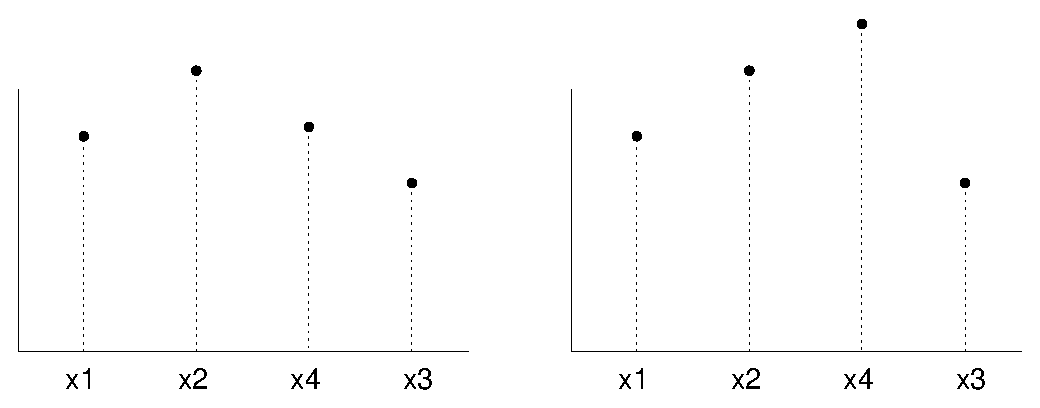
\includegraphics[height=1.5in]{figs/golden2.eps}}

If $f(x_4)$ is less than than $f(x_2)$ (shown on the left), then the
new triple $(x_1, x_2, x_4)$ brackets the maximum. If $f(x_4)$ is
greater than $f(x_2)$ (shown on the right), then $(x_2, x_4, x_3)$
brackets the maximum. Either way the range gets smaller and our
estimate of the optimal value of $x$ gets better.

This method works for almost any value of $x_4$, but some choices
are better than others. In the example, I chose to bisect the
bigger of the ranges $(x_1, x_2)$ and $(x_2, x_3)$.

Here's what that looks like in Octave:

\begin{verbatim}
function res = optimize(V)
  x1 = V(1);
  x2 = V(2);
  x3 = V(3);
  
  fx1 = height_func(x1);
  fx2 = height_func(x2);
  fx3 = height_func(x3);
  
  for i=1:50
    if x3-x2 > x2-x1
      x4 = (x2+x3) / 2;
      fx4 = height_func(x4);
      if fx4 > fx2
        x1 = x2; fx1 = fx2;
        x2 = x4; fx2 = fx4;
      else
        x3 = x4; fx3 = fx4;
      end
    else
      x4 = (x1+x2) / 2;
      fx4 = height_func(x4);
      if fx4 > fx2
        x3 = x2; fx3 = fx2;
        x2 = x4; fx2 = fx4;
      else
        x1 = x4; fx1 = fx4;
      end
    end

    if abs(x3-x1) < 1e-2
      break
    end
  end
  res = [x1 x2 x3];
end
\end{verbatim}

The input variable is a vector that contains three values that bracket
a maximum; in this case they are angles in degrees. {\tt optimize}
starts by evaluating {\tt height\_func} for each of the three values.
We assume that {\tt height\_func} returns the quantity we want to
optimize; for the Green Monster Problem it is the height of
the ball when it reaches the wall.

Each time through the {\tt for} loop the function chooses a value
of {\tt x4}, evaluates {\tt height\_func}, and then updates the
triplet {\tt x1}, {\tt x2} and {\tt x3} according to the results.

After the update, it computes the range of the bracket, {\tt x3-x1},
and checks whether it is small enough. If so, it breaks out of
the loop and returns the current triplet as a result. In the
worst case the loop executes 50 times.

\begin{ex}
I call this algorithm a Silver Section Search because it is almost as
good as a Golden Section Search. Read the Wikipedia page about the
Golden Section Search
(\url{http://en.wikipedia.org/wiki/Golden_section_search}) and then
modify this code to implement it.
\end{ex}

\begin{ex}
You can write functions that take function handles as input
variables, just as {\tt fzero} and {\tt ode45} do.
For example, {\tt handle\_func} takes a function handle called
{\tt func} and calls it, passing {\tt pi} as an argument.

\begin{verbatim}
function res = handle_func(func)
  func(pi)
end
\end{verbatim}

You can call {\tt handle\_func} from the Command Window and pass
different function handles as arguments:

\begin{verbatim}
octave:1> handle_func(@sin)

ans = 0

octave:1> handle_func(@cos)

ans = -1
\end{verbatim}

Modify {\tt optimize} so that it takes a function handle
as an input variable and uses it as the function to be
optimized.
\end{ex}

\begin{ex}
The Octave function {\tt fminsearch} takes a function handle
and searches for a local minimum. Read the documentation for
{\tt fminsearch} and use it to find the optimal launch angle
of a baseball with a given velocity.
\end{ex}


\section{Discrete and continuous maps}

When you solve an ODE analytically, the result is a function,
which you can think of as a continuous map. When you use an
ODE solver, you get two vectors (or a vector and a matrix), which
you can think of as a discrete map.

For example, in Section~\ref{ode45}, we used the following rate
function to estimate the population of rats as a function of time:

\begin{verbatim}
function res = rats(t, y)
  a = 0.01;
  omega = 2 * pi / 365;
  res = a * y * (1 + sin(omega * t));
end
\end{verbatim}

The result from {\tt ode45} is two vectors:

\begin{verbatim}
octave:1> [T, Y] = ode45(@rats, [0, 365], 2);
\end{verbatim}

{\tt T} contains the time values where {\tt ode45} estimated the
population; {\tt Y} contains the population estimates.

Now suppose we would like to know the population on the 180th day
of the year. We could search {\tt T} for the value 180:

\begin{verbatim}
octave:1> find(T==180)

ans = Empty matrix: 0-by-1
\end{verbatim}

But there is no guarantee that any particular value appears in
{\tt T}. We can find the index where {\tt T} crosses 180:

\begin{verbatim}
octave:1> I = find(T>180); I(1)

ans = 23
\end{verbatim}

{\tt I} gets the indices of all elements of {\tt T} greater
than 180, so {\tt I(1)} is the index of the {\em first} one.

Then we find the corresponding value from {\tt Y}:

\begin{verbatim}
octave:1> [T(23), Y(23)]

ans = 184.3451  40.3742
\end{verbatim}

That gives us a coarse estimate of the population on Day 180.
If we wanted to do a little better, we could also find the last value
before Day 180:

\begin{verbatim}
octave:1> [T(22), Y(22)]

ans = 175.2201  36.6973
\end{verbatim}

So the population on Day 180 was between 36.6973 and 40.3742.

But where in this range is the best estimate? A simple option is to
choose whichever time value is closer to 180 and use the corresponding
population estimate. In the example, that's not a great choice
because the time value we want is right in the middle.


\section{Interpolation}

A better option is to draw a straight line between the two points that
bracket Day 180 and use the line to estimate the value in between.
This process is called {\bf linear interpolation}, and Octave provides
a function named {\tt interp1} that does it:

\begin{verbatim}
octave:1> pop = interp1(T, Y, 180)

pop = 38.6233
\end{verbatim}

The first two arguments specify a discrete map from the values in
{\tt T} to the values in {\tt Y}. The third argument is the
time value where we want to interpolate. The result is what
we expected, about halfway between the values that bracket it.

{\tt interp1} can also take a fourth argument that specifies what
kind of interpolation you want. The default is {\tt 'linear'}, which
does linear interpolation. Other choices include {\tt 'spline'}
which uses a spline curve to fit two points on either side,
and {\tt 'cubic'}, which uses piecewise cubic Hermite interpolation.

\begin{verbatim}
octave:1> pop = interp1(T, Y, 180, 'spline')

pop = 38.6486

octave:1> pop = interp1(T, Y, 180, 'cubic')

pop = 38.6491
\end{verbatim}

In this case we expect the spline and cubic interpolations to be
better than linear, because they use more of the data, and we know the
function isn't linear. But we have no reason to expect the spline to
be more accurate than the cubic, or the other way around.
Fortunately, they are not very different.

We can also use {\tt interp1} to project the rat population out
beyond the values in {\tt T}:

\begin{verbatim}
octave:1> [T(end), Y(end)]

ans = 365.0000  76.9530

octave:1> pop = interp1(T, Y, 370, 'cubic')

pop = 80.9971
\end{verbatim}

This process is called {\bf extrapolation}. For time values near
365, extrapolation may be reasonable, but as we go farther into
the ``future,'' we expect them to be less accurate.
For example, here is the estimate we get by extrapolating for a whole
year:

\begin{verbatim}
octave:1> pop = interp1(T, Y, 365*2, 'cubic')

pop = -4.8879e+03
\end{verbatim}

And that's wrong. So very wrong.


\section{Interpolating the inverse function}

We have used {\tt interp1} to find population as a function of time;
by reversing the roles of {\tt T} and {\tt Y}, we can also interpolate
time as a function of population. For example, we might want to know
how long it takes the population to reach 20.

\begin{verbatim}
octave:1> interp1(Y, T, 20)

ans = 133.4128
\end{verbatim}

This use of {\tt interp1} might be confusing if you think of the
arguments as $x$ and $y$. You might find it helpful to think of them
as the range and domain of a map (where the third argument is
an element of the range).

The following plot shows $f$ ({\tt Y} plotted as a function of {\tt T})
and the inverse of $f$ ({\tt T} plotted as a function of {\tt Y}).

\beforefig
\centerline{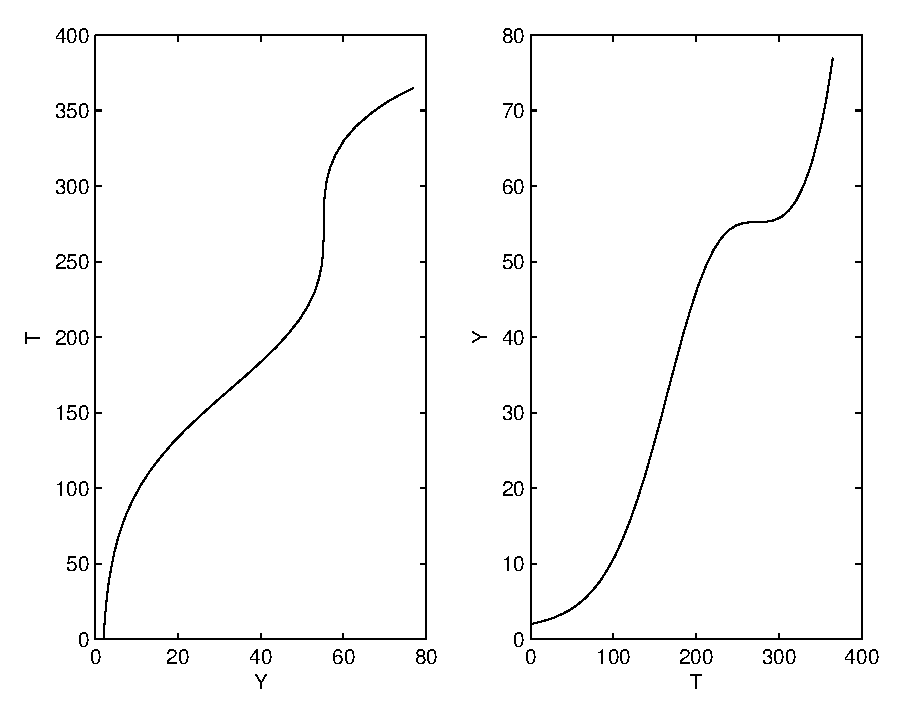
\includegraphics[height=2in,width=4in]{figs/ratplot.eps}}

In this case we can use {\tt interp1} either way because $f$ is
a {\bf single-valued mapping}, which means that for each value in
the domain, there is only one value in the range that maps to it.

If we reduce the food supply so that the rat population decreases
during the winter, we might see something like this:

\beforefig 
\centerline{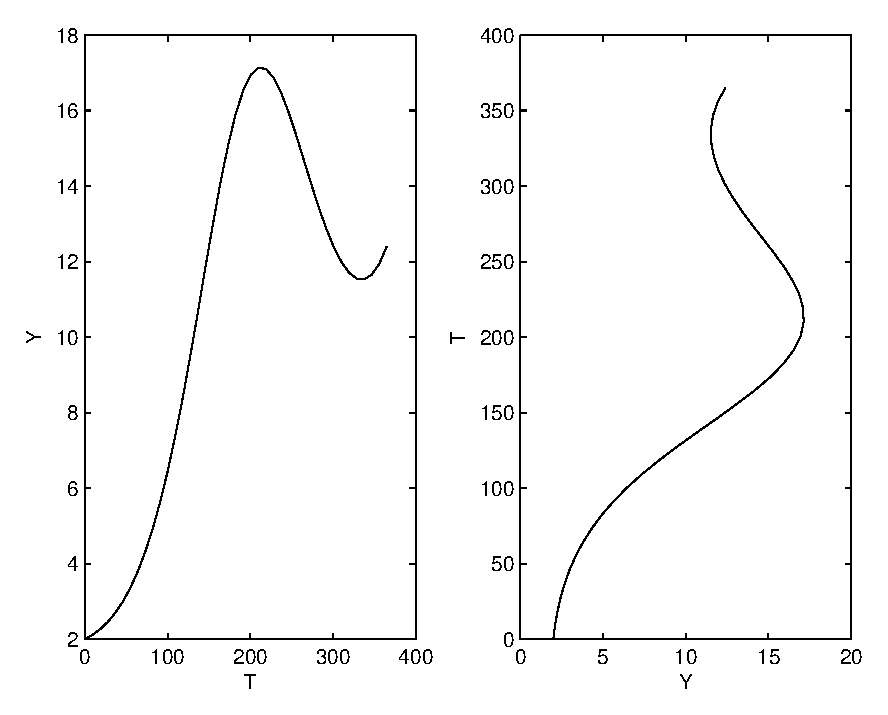
\includegraphics[height=2in,width=4in]{figs/ratplot2.eps}}

We can still use {\tt interp1} to map from {\tt T} to {\tt Y}:

\begin{verbatim}
octave:1> interp1(T, Y, 260)

ans = 15.0309
\end{verbatim}

So on Day 260, the population is about 15, but if we ask on what
day the population was 15, there are two possible answers, 172.44
and 260.44. If we try to use {\tt interp1}, we get the wrong answer:

\begin{verbatim}
octave:1> interp1(Y, T, 15)     

ans = 196.3833        % WRONG
\end{verbatim}

On Day 196, the population is actually 16.8, so {\tt interp1} isn't
even close! The problem is that {\tt T} as a function of {\tt Y} is a
{\bf multivalued mapping}; for some values in the range there are more
than one values in the domain. This causes {\tt interp1} to fail. I
can't find any documentation for this limitation, so that's pretty
bad.


\section{Field mice}

As we've seen, one use of interpolation is to interpret the results
of a numerical computation; another is to fill in the gaps between
discrete measurements.

For example\footnote{This example is adapted from Gerald and Wheatley,
{\em Applied Numerical Analysis}, Fourth Edition, Addison-Wesley,
1989.}, suppose that the population of field mice is governed by this
rate equation:

\[ g : t,y \to ay - b(t) y^{1.7} \]

where $t$ is time in months, $y$ is population, $a$ is a parameter
that characterizes population growth in the absence of limitations,
and $b$ is a function of time that characterizes the effect of the
food supply on the death rate.

Although $b$ appears in the equation as a continuous function, we
might not know $b(t)$ for all $t$. Instead, we might only have discrete
measurements:

\begin{verbatim}
t     b(t)
-     ----
0     0.0070
1     0.0036       
2     0.0011
3     0.0001
4     0.0004
5     0.0013
6     0.0028
7     0.0043
8     0.0056
\end{verbatim}

If we use {\tt ode45} to solve the differential equation, then we
don't get to choose the values of $t$ where the rate function
(and therefore $b$) gets evaluated. We need to provide a function
that can evaluate $b$ everywhere:

\begin{verbatim}
function res = interpolate_b(t)
  T = 0:8;
  B = [70 36 11 1 4 13 28 43 56] * 1e-4;
  res = interp1(T, B, t);
end
\end{verbatim}

Abstractly, this function uses a discrete map to implement a
continuous map. 

\begin{ex}
Write a rate function that uses
{\tt interpolate\_b} to evaluate $g$ and then
use {\tt ode45} to compute the population of field mice
from $t=0$ to $t=8$ with an initial population of 100 and
$a=0.9$.

Then modify {\tt interpolate\_b} to use spline interpolation
and run {\tt ode45} again to see how much effect the interpolation
has on the results.
\end{ex}

\section{Glossary}

\begin{description}

\item[interpolation:] Estimating the value of a function using
known values on either side.

\item[extrapolation:] Estimating the value of a function using
known values that don't bracket the desired value.

\item[single-valued mapping:] A mapping where each value in the
range maps to a single value in the domain.

\item[multivalued mapping:] A mapping where at least one value in
the range maps to more than one value in the domain.

\end{description}


\section{Exercises}

\begin{ex}
\label{golf}

A golf ball\footnote{See
\url{http://en.wikipedia.org/wiki/Golf_ball}.} hit with backspin
generates lift, which might increase the range, but the energy that
goes into generating spin probably comes at the cost of lower initial
velocity. Write a simulation of the flight of a golf ball and use it
to find the launch angle and allocation of spin and initial velocity
(for a fixed energy budget) that maximizes the horizontal range of the
ball in the air.

The lift of a spinning ball is due to the Magnus force\footnote{See
\url{http://en.wikipedia.org/wiki/Magnus_effect}.}, which is
perpendicular to the axis of spin and the path of flight. The
coefficient of lift is proportional to the spin rate; for a ball
spinning at 3000 rpm it is about 0.1. The coefficient of drag of a
golf ball is about 0.2 as long as the ball is moving faster than 20 m/s.
\end{ex}
